\documentclass[openany]{book}
\input{notes_white}
\usepackage{mathtools}
\usepackage{pgfplots}
\settitle{Biology Lab Manual}
\begin{document}
\title{\Large{\underemphasise{Biophysics - Expt 2}} \\ \vspace{5pt}
\large{Observing and Analysing the Diffusion of Single Particles}}
\author{Eklavya Raman \\ \vspace{5pt} er24ms024@iiserkol.ac.in \\ \vspace{5pt}
\and Shrey Patnaik \\ \vspace{5pt} sp24ms174@iiserkol.ac.in \\ \vspace{5pt}}
\date{\today}
\maketitle
\begin{center}
    \textbf{Abstract}
\end{center}
    This experiment focuses on observing and analyzing the diffusion of single particles in a fluid medium. By tracking the motion of individual particles over time, we can gain insights into their diffusion behavior and calculate the diffusion coefficient. The analysis is performed using Image-J software, which allows us to extract particle trajectories and compute relevant statistical measures. The principle of diffusion is based on the random motion of particles, leading to an even distribution over time. By measuring the displacement of particles at different time intervals, we can calculate the diffusion coefficient using the mean squared displacement (MSD) method.
\subsubsection{Aim}
To observe and analyze the diffusion of single particles.
\subsubsection{Apparatus}
\begin{itemize}
    \item Microscope with camera attachment
    \item Microscope slides and cover slips
    \item Polystyrene beads (1 $\mu$m diameter)
    \item Water
    \item Image-J software
    \item Pipette
\end{itemize}
\subsubsection{Working Principle}
The diffusion of particles in a fluid medium is governed by Brownian motion, which describes the random movement of particles due to collisions with the molecules of the surrounding fluid. By tracking the motion of individual particles over time, we can analyze their trajectories and calculate the diffusion coefficient (D) using the mean squared displacement (MSD) method. The MSD is defined as:
$$\boxed{MSD(\tau) = \langle [x(t + \tau) - x(t)]^2 + [y(t + \tau) - y(t)]^2 \rangle}$$
where $\tau$ is the time lag, and the angle brackets denote an average over all particles and time points. For two-dimensional diffusion, the diffusion coefficient can be estimated from the MSD using the relation:
$$\boxed{D = \frac{MSD(\tau)}{4\tau}}$$
We can also use the formula - 
$$\boxed{D = \frac{k_B T}{6 \pi \eta r}}$$
where $k_B$ is the Boltzmann constant, $T$ is the absolute temperature, $\eta$ is the dynamic viscosity of the fluid, and $r$ is the radius of the particle.
\subsubsection{Experimental Procedure}
\underemphasise{Sample Cell Preparation:}
\begin{enumerate}
\item Take a clean microscope slide. Cut two strips of parafilm, remove the paper and place on top of the slide, parallel to each other and about 1.5 cm apart.
\item Take a 18/22 mm cover slip and place it on top of the parafilm strips.
\item Gently press the sandwich to ensure that the parafilm sticks to the slide and cover slip.
\item Place on top of an aluminium foil on a heater pressing the sandwich gently to melt the parafilm and seal the edges.
\item Let it cool for a few minutes.
\end{enumerate}
\underemphasise{Putting in bead mix: }
\begin{enumerate}
    \item Introduce 20-50 $\mu$L of the bead solution on one side of the cover slip using a pipette.
    \item Use a tissue paper to wick away excess liquid from the other side of the cover slip. This will create a thin film of liquid between the slide and cover slip.
    \item Keep the sample-cell on the microscope stage. 
    \item Place a small drop of oil on the top of the cover slip and lower the 100X oil-immersion objective into the oil drop.
    \item Focus on the beads using the fine adjustment knob.
    \item Adjust the illumination to get a clear view of the beads.
    \item Capture a video of the beads diffusing in the water.
    \item Stop the video capture after a few minutes.
    \item Analyze the video using Image-J to extract the diffusion data.
\end{enumerate}
\underemphasise{Analysis using Image-J}
\begin{enumerate}
\item Extract frames from the video file using a python script or any other method.
\item Open a frame in Image-J and set the scale using a known length (e.g., the diameter of a bead).
\item Estimate the average diameter of the beads in pixels using the line tool and the "Measure" function.
\item Using the working formula, calculate an estimate for the diffusion coefficient (D) based on the bead diameter, temperature, and viscosity of water.
\end{enumerate}
\subsubsection{Observations and Results}
\begin{figure}[H]
    \centering
    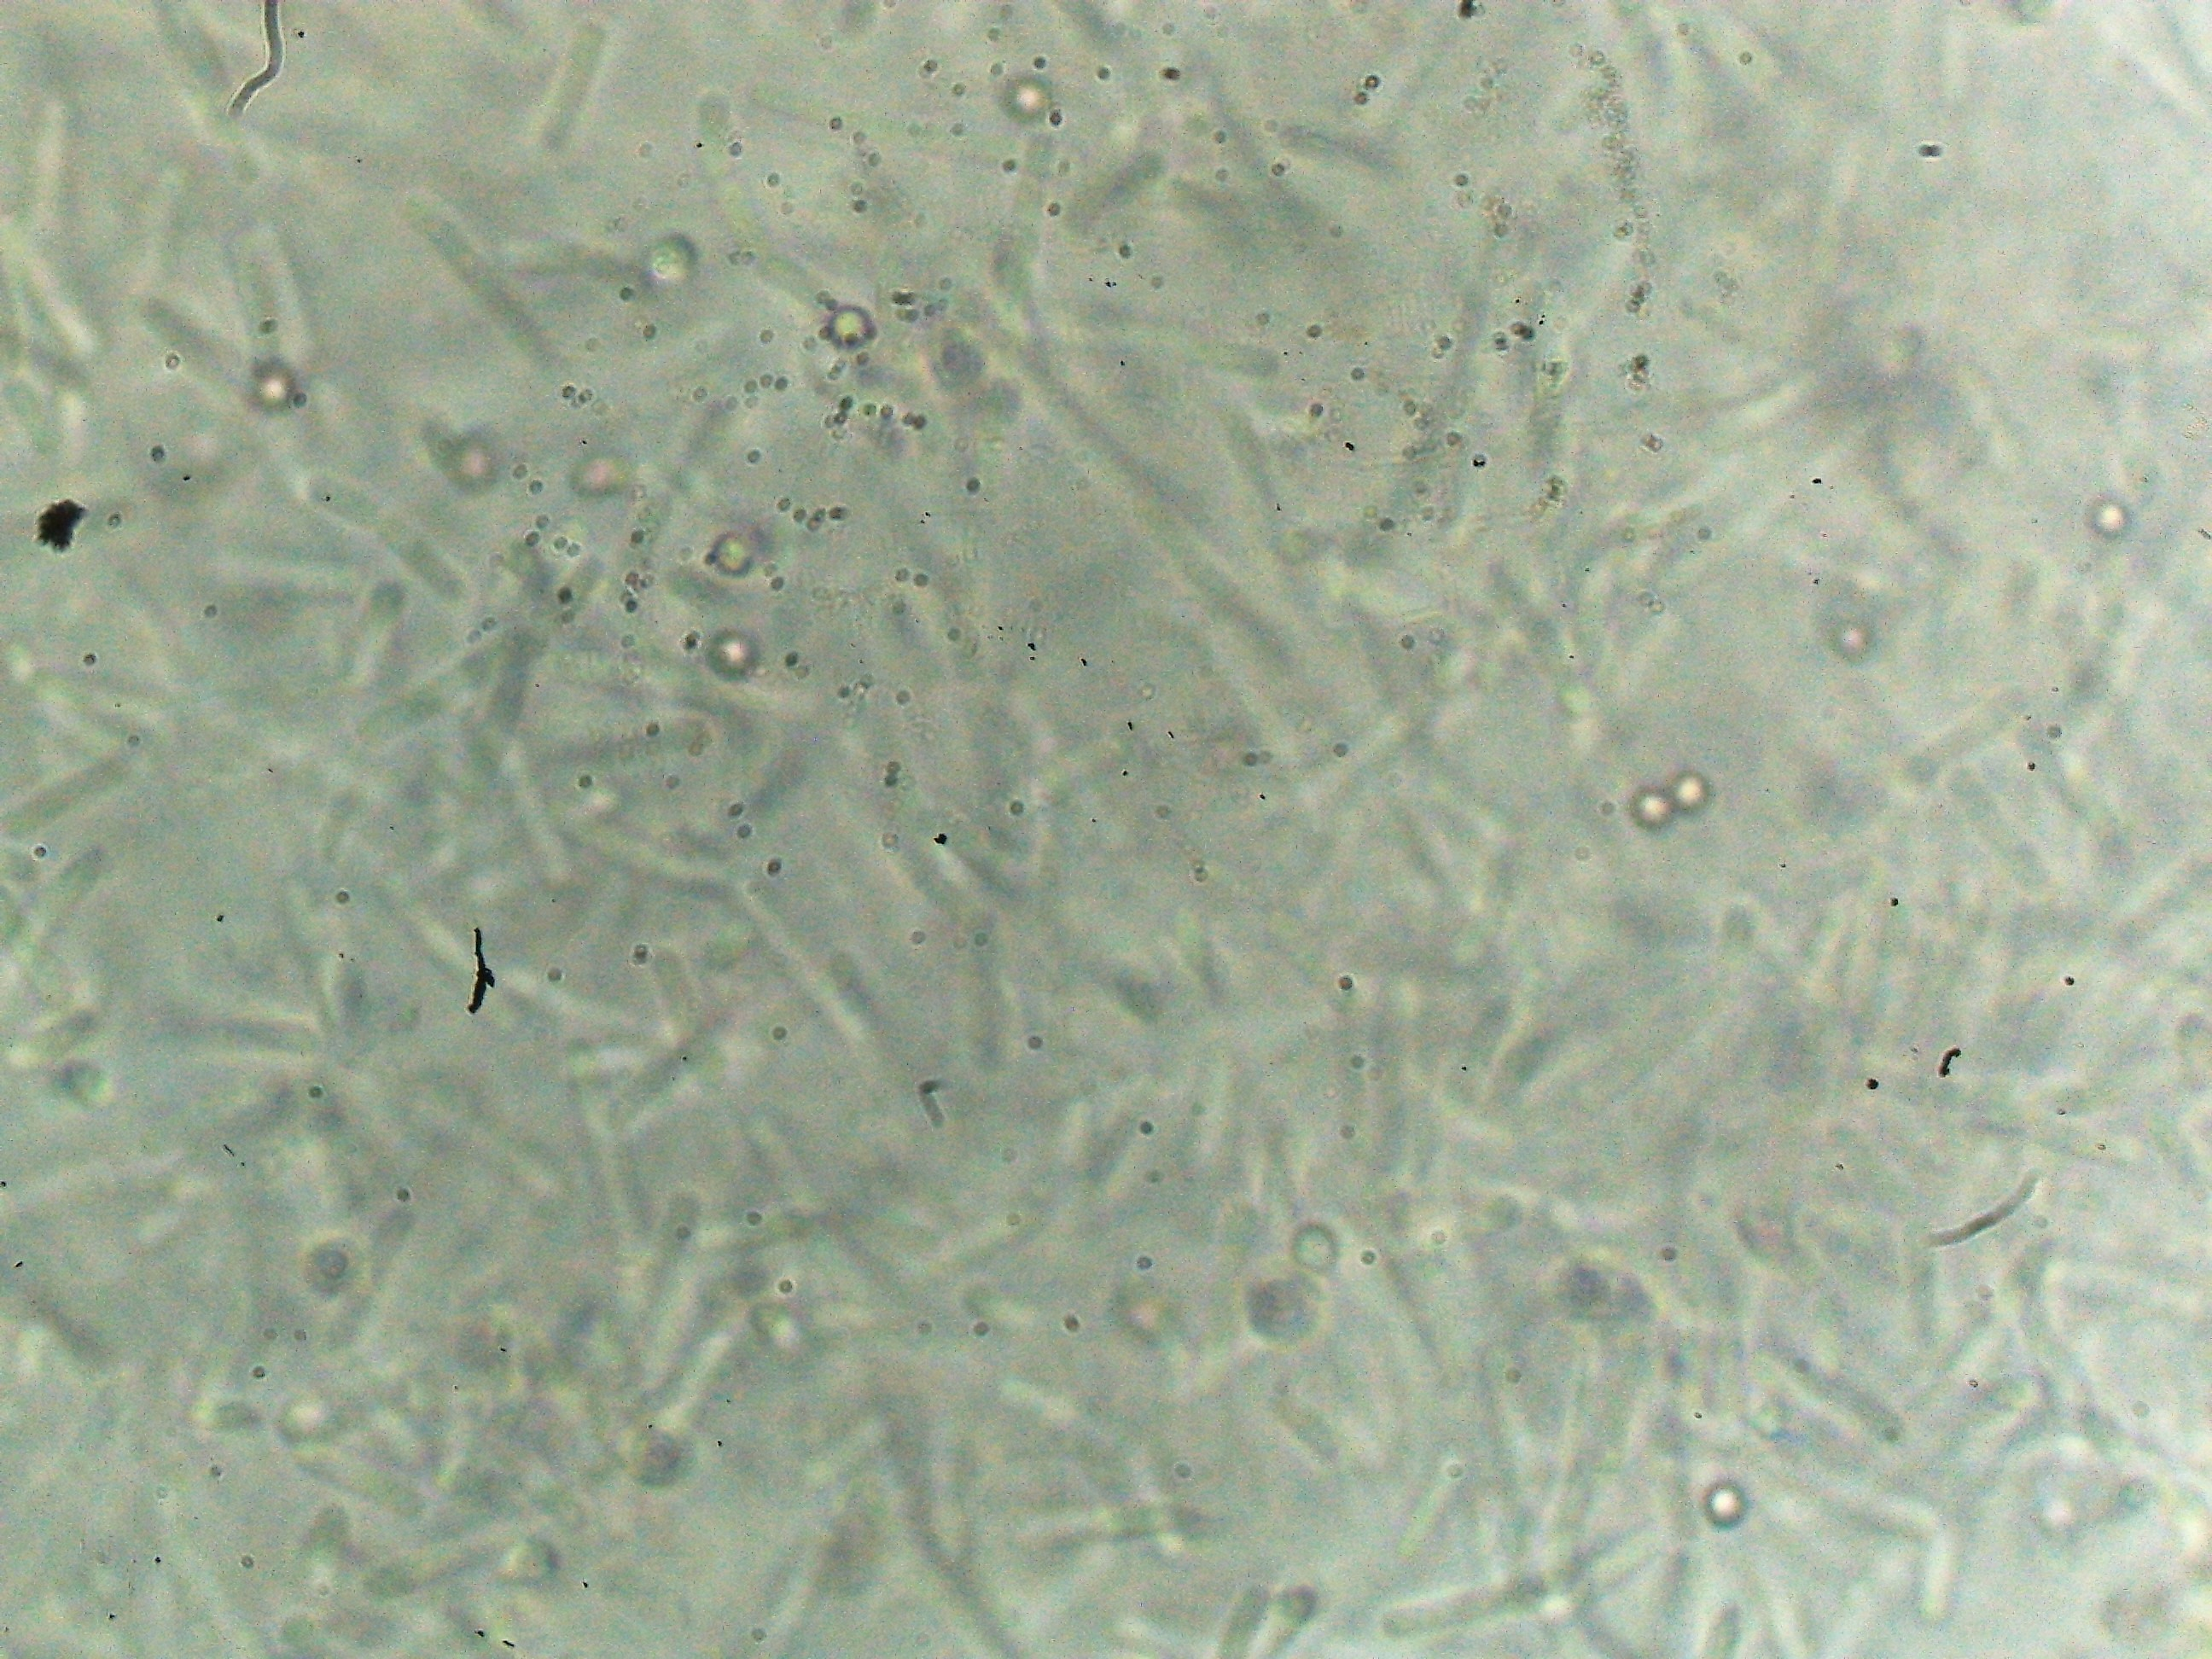
\includegraphics[width=0.5\textwidth]{images/WIN_20250820_15_31_07_Pro.jpg}
    \caption{Microscope Image of 5 $\mu$m Polystyrene Beads in Water}
\end{figure}
We find the measurement of the bead diameter to be - 
\begin{figure}[H]
    \centering
    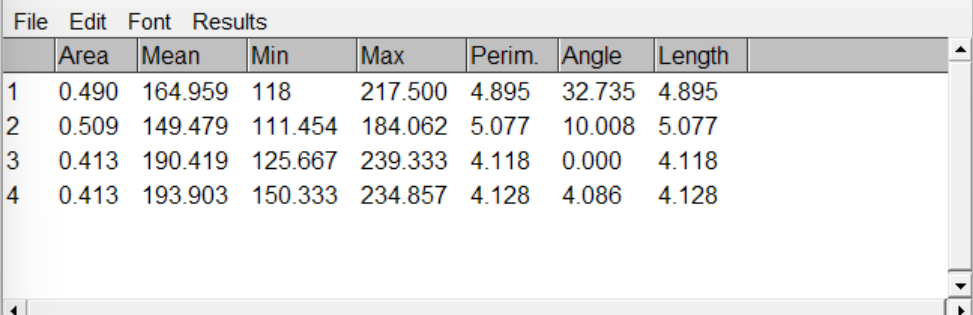
\includegraphics[width=0.5\textwidth]{images/Screenshot 2025-09-24 223336.png}
    \caption{Measurement of Bead Diameter using Image-J}
\end{figure}
The average radius then is - 
$$d = \frac{4.895 + 5.077 + 4.118 + 4.128}{4} = 4.5545 \mu m$$
Thus, the radius $d = 2.27725 \mu m = 2.27725 \times 10^{-6} m$. \\
Assuming room temperature $T = 298 K$ and viscosity of water $\eta = 0.89 \times 10^{-3} Pa \cdot s$, we can calculate the diffusion coefficient using the Stokes-Einstein equation:
$$D = \frac{k_B T}{6 \pi \eta r}$$
where $k_B = 1.38 \times 10^{-23} J/K$ is the Boltzmann constant. Plugging in the values, we get:
$$D = \frac{1.38 \times 10^{-23} \times 298}{6 \pi \times 0.89 \times 10^{-3} \times 2.27725 \times 10^{-6}}$$
$$D \approx 1.08 \times 10^{-13} m^2/s$$

This value is an estimate of the diffusion coefficient for the 5 $\mu$m polystyrene beads in water at room temperature. \\
\textbf{Note:} The actual diffusion coefficient may vary based on experimental conditions, and further analysis using the MSD method from the tracked particle trajectories can provide a more accurate measurement.

\subsubsection{Conclusion}
In this experiment, we successfully observed and analyzed the diffusion of single polystyrene beads in water using a microscope and Image-J software. By measuring the bead diameter and applying the Stokes-Einstein equation, we estimated the diffusion coefficient to be approximately $1.08 \times 10^{-12} m^2/s$. This value provides insight into the diffusion behavior of the beads in the fluid medium. Further analysis using the mean squared displacement (MSD) method from tracked particle trajectories can enhance the accuracy of our diffusion coefficient measurement. Overall, this experiment demonstrates the principles of Brownian motion and diffusion in a practical setting.
\end{document}